\begin{note}
    Теоремы о неопределенности \hyperlink{zero_on_zero_th}{$\frac{0}{0}$} и \hyperlink{inf_on_inf_th}{$\frac{\infty}{\infty}$}
    справедливы также при замене $x \to a+0$ на $x \to b-0$, $x \to x_0$, $x \to \pm \infty$.
\end{note}

\begin{proof} (для случая, $a = -\infty$)\\
    Без ограничения общности $b < 0$.
    Рассмотрим на $(0, -\frac{1}{b})$ функции
    $\phi(t) = f(-\frac{1}{t})$, $\psi(t) = g(-\frac{1}{t})$.
    Функции $\phi$, $\psi$ дифференцируемы на $(0, -\frac{1}{b})$
    и $\psi'(t) = g'(-\frac{1}{t}) \cdot  \frac{1}{t^2} \neq 0$
    и по свойству предела композиции $\lim_{t \to +0} \phi(t) = \lim_{x \to -\infty} f(x)$, $\lim_{t \to +0} \psi(t) = \lim_{x \to -\infty} g(x)$
    и существует $\lim_{t \to +0} \frac{\phi'(t)}{\psi'(t)} = \lim_{x \to -\infty} \frac{f'(x)}{g'(x)}$.
    Тогда по доказанному существует $\lim_{t \to +0} \frac{\phi(t)}{\psi(t)} = \lim_{t \to +0} \frac{\phi'(t)}{\psi'(t)}$ и, значит, существует $\lim_{x \to -\infty} \frac{f(x)}{g(x)} = \lim_{x \to -\infty} \frac{f'(x)}{g'(x)}$.
\end{proof}

\begin{example}
    1) $\lim_{x \to +\infty} \frac{\ln x}{x^{\alpha}} = 0 \forall \alpha > 0$.\\
    Так как $\lim_{x \to +\infty} \frac{\ln x}{x^{\alpha}} = \lim_{x \to +\infty} \frac{1/x}{\alpha x^{\alpha-1}} = \lim_{x \to +\infty} \frac{1}{\alpha x^{\alpha} = 0}$\\
    2) $\lim_{x \to +\infty} \frac{x^{\alpha}}{a^{x}} = 0$ при $\alpha > 0$ и $a > 1$.\\
    Имеем $\lim_{x \to +\infty} \frac{x}{a^{x}} = \lim_{x \to +\infty} \frac{1}{a^{x} \ln a} = 0$.\\
    Так как $\frac{x^{\alpha}}{a^{x}} = (\frac{x}{(a^{\frac{1}{\alpha}})^x})^{\alpha}$ и $\lim_{y \to +\infty} y^{\alpha} = 0$, то по свойству предела композиции $\lim_{x \to +\infty} (\frac{x}{(a^{\frac{1}{\alpha}})^x})^{\alpha} = 0$.\\
    Вывод: степенная функция при $x \to +\infty$ растет быстрее логарифмической, но медленнее показательной функции.
\end{example}

\begin{problem}
    Покажите, что существует $\lim_{x \to +\infty} \frac{x+ \sin x}{x}$,
    однако его нельзя найти по правилу Лопиталя.
\end{problem}

\subsection{Производные высших порядков}
Производные высших порядков определяются индуктивно.

\begin{definition}
    Пусть $n \in \N$. Положим $f^{(1)} = f'$.
    Если $n > 1$, функция $f^{(n-1)}$ определена в некоторой окрестности точки $a$
    и дифференцируема в самой точке $a$, то функция $f$ называется
    \textit{дифференцируемой n раз} в точке $a$, и ее производная $n$-ого порядка
    в точке $a$ определяется равенством $f^{(n)}(a) = (f^{(n-1)})'(a)$.
    Считаем также $f^{(0)} = f$.    
\end{definition}

Функция $f$ называется $n$ раз дифференцируемой на множестве $E$,
если она $n$ раз дифференцируема в каждой точке из $E$. 

\begin{note}
    Если $n > 1$, то существование производной $n$-ого порядка в точке $a$
    влечет существование производных $n-1$-ого порядка в некоторой окрестности точки $a$.
\end{note}

Ввиду линейности дифференцирования, по индукции устанавливается, что $(\alpha f + \beta g)^{(n)} = \alpha f^{(n)} + \beta g^{(n)}$, если $\exists f^{(n)}, g^{(n)}$.
Для произведения справедлива следующая формула.

\begin{theorem} (формула Лейбница)\\
    Если $f$ и $g$ дифференцируемы $n$ раз в точке $x$,
    то в точке $x$ также дифференцируема $n$ раз функция $f \cdot g$,
    причем справедлива формула: \[(f\cdot g)^{(n)} (x) = \sum_{k = 0}^{n} C_{n}^{k}f^{(k)}(x)g^{(n-k)}(x)\]
\end{theorem}

\begin{proof}
    Докажем индукцией по $n$. При $n = 1$ равенство известно $(fg)'(x) = f'(x)g(x) + f(x)g'(x)$.
    Предположим, утверждение верно для $n$, тогда (опуская аргумент $x$)
    \[(fg)^{(n+1)} = ((fg)^{n})' = \]
    \[= (\sum_{k = 0}^{n} C_{n}^{k}f^{(k)}(x)g^{(n-k)}(x))' = \]
    \[= \sum_{k = 0}^{n} C_{n}^{k}f^{(k+1)}(x)g^{(n-k)}(x) + \sum_{k = 0}^{n} C_{n}^{k}f^{(k)}(x)g^{(n-k+1)}(x) = \]
    \[= f^{(n+1)}g + \sum_{k = 1}^{n} C_{n}^{k-1}f^{(k)}(x)g^{(n+1-k)}(x) + \sum_{k = 1}^{n} C_{n}^{k}f^{(k)}(x)g^{(n+1-k)}(x) + fg^{(n+1)} = \]
    \[= \sum_{k = 1}^{n} (C_{n}^{k-1} + C_{n}^{k})f^{(k)}(x)g^{(n+1-k)}(x) + f^{(n+1)}g + fg^{(n+1)} =
    \sum_{k = 0}^{n+1} C_{n+1}^{k}f^{(k)}(x)g^{(n+1-k)}(x) \]
    Так как $C_{n}^{k-1} + C_{n}^{k} = C_{n+1}^{k}$.
\end{proof}

\begin{corollary} (формула Бинома)\\
    \[(a+b)^n = \sum_{k = 0}^{n} C_{n}^{k}a^kb^{n-k}\]
    $u = e^a, v = e^b$, тогда $((uv)^x)^{(n)} = (uv)^x\ln^nuv = (uv)^x(lnu+lnv)^n$\\
    с другой стороны $(u^x\cdot v^x)^{(n)} = \sum_{k = 0}^{n}C_n^k(u^k\cdot \ln^ku)(v^{(n-k)}\cdot \ln^{(n-k)}v) = (uv)^x\sum_{k = 0}^{n}C_n^k\ln^ku\ln^{(n-k)}v$
\end{corollary}

\subsection{Формула Тейлора}

\begin{definition}
    Пусть $n \in \N$ и функция $f$ дифференцируема $n$ раз в точке $a$.
    Тогда равенство:
    \[f(x) = \sum_{k = 0}^{n} \frac{f^{(k)}(a)}{k!}(x-a)^k + r_n(x)\]
    называется \textit{формулой Тейлора} порядка $n$ функции $f$ в точке $a$.\\
    При этом многочлен $P_n(x) = P_{n, a, f}(x) = \sum_{k = 0}^{n} \frac{f^{(k)}(a)}{k!}(x-a)^k$
    называется \textit{многочленом Тейлора},
    $r_n(x) = r_{n, a, f}(x)$ - \textit{остаточным членом}.
\end{definition}

\begin{example}
    Если $P(x) = \sum_{k = 0}^{n}c_k(x-a)^k$,
    то $P^{(m)}(x) = \sum_{k = m}^{n} \frac{k!}{(k-m)!}c_k(x-a)^{k-m}, 0 \leq m \leq n$,
    поэтому $P^{(m)}(a) = m!c_m$. Таким образом, $P(x) = \sum_{k = 0}^{n} \frac{P^{(k)}(a)}{k!}(x-a)^k = \sum_{k = 0}^{n}c_k(x-a)^k$
    - формула Тейлора многочлена $P$.
\end{example}

\begin{theorem} (остаточный член в форме Пеано)\\
    Пусть $n \in \N$ и функция $f$ дифференцируема $n$ раз в точке $a$.
    Тогда \[f(x) = \sum_{k = 0}^{n} \frac{f^{(k)}(a)}{k!}(x-a)^k + o((x-a)^n), x \to a\]
    то есть $r_n(x) = o((x-a)^n)$ при $x \to a$.
\end{theorem}

\begin{proof}
    Пусть $P_n(x) = \sum_{k = 0}^n \frac{f^{(k)}(a)}{k!}(x-a)^k$,
    тогда $P^{(k)}(a) = f^{(k)}(a), 0 \leq k \leq n$.
    Поэтому для остаточного члена $r_n(x) = f(x) - P_n(x)$
    выполнено $r_n(a) = r_n'(a) = \dots = r_n^{(n)}(a) = 0$.
    По \hyperlink{zero_on_zero_th}{правилу Лопиталя}
    \[\lim_{x \to a} \frac{r_n(x)}{(x-a)^n} = \lim_{x \to a} \frac{r_n'(x)}{n(x-a)^{n-1}} = \dots = \lim_{x \to a} \frac{r_n^{(n-1)}(x)}{n!(x-a)}\]
    Последний предел существует по определению $n$-й производной в точке $a$:
    \[\lim_{x \to a} \frac{r_n^{(n-1)}(x)}{n!(x-a)} = \frac{1}{n!}\lim_{x \to a} \frac{r_n^{(n-1)}(x) - r_n^{(n-1)}(a)}{(x-a)} = \frac{r_n^{(n)}(a)}{n!} = 0\]
    следовательно, $r_n(x) = o((x-a)^n)$ при $x \to a$
\end{proof}

\begin{corollary} (условия экстремума)\\
    Пусть $n \in \N$, функция f дифференцируема $n$ раз в точке $a$ и $f'(a) = \dots = f^{(n-1)}(a) = 0$,
    но $f^{(n)}(a) \neq 0$. Тогда
    \begin{enumerate}
        \item если $n$ четно и $f^{(n)}(a) < 0$ ($f^{(n)}(a) > 0$), то $a$ является точкой
        строгого локального максимума (минимума) функции $f$.
        \item если $n$ нечетно, то $a$ не является точкой локального
        экстремума функции $f$.
    \end{enumerate}
\end{corollary}

\begin{proof}
    По предыдущей теореме
    \[f(x) - f(a) = \frac{f^{(n)}(a)}{n!}(x-a)^n + o((x-a)^n) =\]
    \[= (\frac{f^{(n)}(a)}{n!} + \alpha(x))\cdot (x-a)^n\]
    где $\alpha(x) \to 0$ при $x \to a$. Найдется такое $\delta > 0$,
    что $|\alpha(x)| < |\frac{f^{(n)}(a)}{n!}| \ \forall x \in \mathring{B}_{\delta}(a)$,
    поэтому $sign(\frac{f^{(n)}(a)}{n!} + \alpha(x)) = sign(f^{(n)}(a)) \forall x \in \mathring{B}_{\delta}(a)$,
    и значит, в $\mathring{B}_{\delta}(a)$ $\ sign(f(x) - f(a)) = sign(f^{(n)}(a)(x-a)^n)$.\\
    Что в 1 случае дает одинаковые знаки при $x < a$ и $x > a$. И во втором - разные.
\end{proof}

\begin{theorem}{О единственности разложения}\\
    Пусть $p_{1}(x), p_{2}(x)$ -- такие многочлены степени $\leq n$, что $f(x) - p_{1}(x) = o((x-a)^{n})$
    и $f(x) - p_{2}(x) = o((x-a)^{n}), x \to a$. Тогда $p_{1}(x) = p_{2}(x)$.
\end{theorem}

\begin{proof}
    Положим $q(x) = p_{1}(x) - p_{2}(x)$, тогда $q(x) = o((x-a)^{n})$. Покажем, что $q(x)$ -- нулевой многочлен.\\
    Пусть $q(x) = c_{0} + c_{1}(x-a) + ... + c_{n}(x-a)^{n}$. Предположим, что $\exists c_{i} \neq 0$. Тогда положим $j = \min\{k: c_{k} \neq 0\}$. Поделим равенство на $(x-a)^{j}$ получим $q(x) = o((x-a)^{n-j})$. Перейдем к пределу при $x \to a$, тогда $c_{j} = 0$. Противоречие.
\end{proof}

\begin{corollary}
    Если функция $f$ дифференцируема $n$ раз в точке $a$ и $f(x) = \sum\limits_{k = 0}^{n} c_{k}(x-a)^{k} + o((x - a)^{n}), x \to a$. Тогда $c_{k} = \frac{f^{(k)}(a)}{k!}, k = 0, 1, ...$.
\end{corollary}

Покажем, как полученное следствие позволяет восстановить разложение функции по разложению ее производной.

\begin{note}
    Пусть функция $f$ дифференцируема $n + 1$ раз в точке $a$ и \\ $f'(x) = \sum\limits_{k = 0}^{n} c_{k} (x-a)^{k} + o((x - a)^{n}), x \to a$. Тогда 
    \[f(x) = f(a) + \sum\limits_{k = 0}^{n}\frac{c_{k}}{k + 1} (x-a)^{k + 1} + o((x - a)^{n+1}), x \to a\]
\end{note}

\begin{proof}
    Выпишем формулу Тейлора функции $f$: $f(x) = f(a) + \sum\limits_{k = 0}^{n}\frac{f^{(k+1)}(a)}{(k + 1)!} (x-1)^{k + 1} + o((x - a)^{n+1}), x \to a$. Из разложения $f'$ по следствию имеем: $c_{k} = \frac{(f')^{(k)}(a)}{k!} \lra f^{(k+1)}(a) = c_{k}k!, k = 0, 1, ...$. Откуда следует представление $f$.
\end{proof}

Формула Тейлора для точки $a = 0$ называется формулой Маклорена.

\subsection{Основные разложения.}
    $1)$ Если $f(x) = e^{x}$, то $f^{(k)}(0) = e^{0} = 1, k \in \N$. Следовательно, 
    \[e^{x} = \sum_{k=0}^{n}\frac{x^{k}}{k!} + o(x^{n}), x \to 0\]
    $2)$ Если $f(x) = \sin(x)$. Тогда (по индукции) $f^{(n)}(x) = \sin(x + \frac{\pi}{2}n), n \in \N$. Поэтому $f^{(2k)}(0) = 0, f^{(2k+1)}(0) = (-1)^{k}$. Следовательно, 
    \[\sin(x) = \sum_{k = 0}^{n} \frac{(-1)^{k} x^{2k+1}}{(2k+1)!} + o(x^{2n+2}), x \to 0\]
    $3)$ Если $f(x) = \cos(x)$. Тогда (по индукции) $f^{(n)}(x) = \cos(x + \frac{\pi}{2}n), n \in \N$. Поэтому $f^{(2k)}(0) = (-1)^{k}, f^{(2k + 1)}(0) = 0$. Следовательно, 
    \[\cos(x) = \sum_{k = 0}^{n} \frac{(-1)^{k} x^{2k}}{(2k)!} + o(x^{2n+1}), x \to 0\]
    $4)$ Если $f(x) = (1+x)^{\alpha}, \alpha \in \R$, то $f^{(k)}(x) = \alpha \cdot (\alpha - 1) \cdot ... \cdot (\alpha - k + 1)(1+x)^{\alpha - k}$. \\
    Положим $c_{\alpha}^{0} = 1, c_{\alpha}^{k} = \frac{\alpha \cdot (\alpha - 1) \cdot ... \cdot (\alpha - k + 1)}{k!}$. Следовательно, 
    \[(1+x)^{\alpha} = \sum_{k = 0}^{n} c_{\alpha}^{k}x^{k} + o(x^{n}), x \to 0\]
    В частности $\frac{1}{1+x} = \sum_{k = 0}^{n} (-1)^{k} x^{k} + o(x^{n}), x \to 0$. \\
    $5)$ Если $f(x) = \ln(1+x)$, то $f(0) = 0$, $f^{(k)}(x) = \frac{(-1)^{k-1}(k-1)!}{(1+x)^{k}}$. Следовательно,
    \[\ln(1+x) = \sum_{k = 0}^{n} \frac{(-1)^{k-1}}{k}x^{k} + o(x^{n}), x \to 0\]

\begin{example}
    Представьте формулой Маклорена $e^{\sin(x)}$ до $o(x^{4})$.
\end{example}

\begin{proof}
    Пусть $P$ -- многочлен Тейлора порядка 4 функции $exp$ в точке $a = 0$. Делая замену $w = \sin(x)$ в пределе $\lim_{w \to 0}\frac{e^{w} - P(w)}{w^{4}} = 0$, приходим к равенству
    \[e^{\sin(x)} = 1 + \sin(x) + \frac{\sin^{2}(x)}{2} + \frac{\sin^{3}(x)}{6} + \frac{\sin^{4}(x)}{24} + o(\sin^{4}(x)), x \to 0\]
    Поскольку $\sin(x) ~ x$, то $o(w^{4}) = o(x^{4})$ при $x \to 0$. Далее, используя представление $\sin(x) = x - \frac{x^{3}}{6} + o(x^{4})$, имеем
    \[w^{2} = x^{2} - \frac{x^{4}}{3} + o(x^{4})\]
    \[w^{3} = x^{3} + o(x^{4})\]
    \[w^{4} = x^{4} + o(x^{4})\]
    После приведения подобных слагаемых, получаем требуемое представление:
    \[e^{\sin(x)} = 1 + x + \frac{x^{2}}{2} - \frac{x^{4}}{8} + o(x^{4}), x \to 0\]
\end{proof}

\begin{theorem} {Остаточный член в формуле Лагранжа.}\\
    Пусть функция $f$ дифференцируема $n+1$ раз на $(\alpha , \beta)$ и $a \in (\alpha, \beta)$. Тогда для любой точки $x \in (\alpha, \beta),\ x \neq a$, найдется точка $c$, лежащая между $a$ и $x$, что
    \[f(x) = \sum_{k = 0}^{n}\frac{f^{(k)}(a)}{k!}(x-a)^{k} + \frac{f^{(n+1)}(c)}{(n+1)!}(x-a)^{n+1}\]
    т.е. $r_{n}(x) = \frac{f^{(n+1)}(c)}{(n+1)!}(x-a)^{n+1}$.
\end{theorem}

\begin{proof}
    Пусть для определенности $x > a$. Рассмотрим функции $\phi (t) = f(t) + f'(t)(x-t) + ... + \frac{f^{(n)}(t)}{n!}(x-t)^{n}$, $\psi (t) = (x-t)^{n+1}$. Функции $\phi$ и $\psi$ дифференцируемы на $[a,x]$, $\phi'(t) = \frac{f^{(n+1)}(t)}{n!}(x - t)^{n}$ и $\psi'(t) = -(n+1)(x-t)^{n}$, причем $\psi' \neq 0$ на $(a, x)$. Тогда по \hyperlink{koshi_o_srednem}{теореме Коши} найдется такая точка $c \in (a,x)$, что
    \[\frac{\phi(x) - \phi(a)}{\psi(x) - \psi(a)} = \frac{\phi'(c)}{\psi'(c)} \lra \frac{f(x) - \sum\limits_{k=0}^{n}\frac{f^{(k)}(a)}{k!}(x-a)^{k}}{-(x-a)^{n+1}} = \frac{\frac{f^{(n+1)}(c)}{n!}(x - c)^{n}}{-(n+1)(x-c)^{n}},\]
    откуда получаем, что $r_{n}(x) = \frac{f^{(n+1)(c)}}{(n+1)!}(x-a)^{n+1}$.
\end{proof}

\begin{note}
    Если вместо $\psi$ взять $\psi(t) = x - t$, то получим $r_{n}(x) = \frac{f^{(n+1)}(c)}{n!}(x-c)^{n}(x-a)$ (остаточный член в форме Коши). Меняя $\psi$ можно получать другие формы для $r_{n}$.
\end{note}

\subsection{Выпуклые функции}

\begin{definition}
    Пусть $f$ определена на промежутке $I$. Функция $f$ называется \textit{выпуклой} (или выпуклой вниз) на $I$, если для любых $x_{1}, x_{2} \in I, x_{1} \neq x_{2}$ и $t \in (0,1)$ выполнено
    \[f((1-t)x_{1} + tx_{2}) \leq (1-t)f(x_{1}) + tf(x_{2}).\]
    Если неравенство строгое, то говорят, что $f$ \textit{строго выпукла} на $I$. Функция $f$ называется \textit{вогнутой}(или выпуклой вверх) на $I$, если функция $(-f)$ выпукла на $I$. Аналогично определяется строгая вогнутость.
\end{definition}

\begin{note}
    Геометрический смысл.\\
    Выпуклость означает, что график функции лежит \textit{не выше} любой своей хорды.
    \begin{center}
        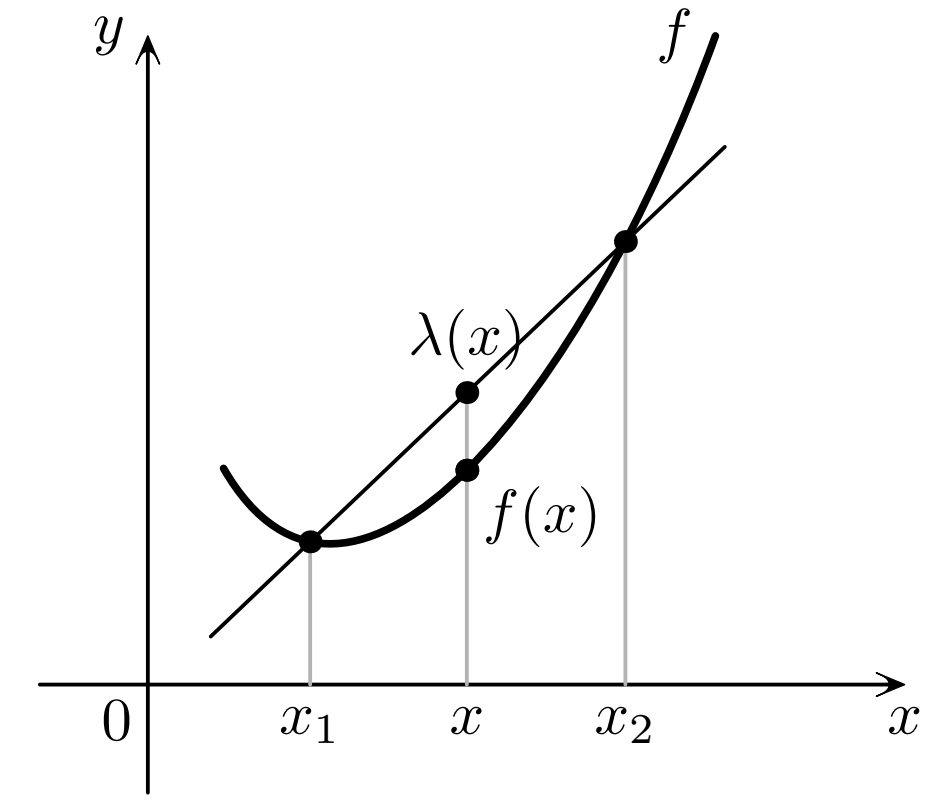
\includegraphics[width=0.4\textwidth]{ex2.png}
    \end{center}
\end{note}

\begin{example}
    \begin{enumerate}
        \item $f(x)= kx+b \ (k,b \in \R)$ -- одновременно выпукла и вогнута на любом промежутке.
        \item $f(x) = x^{2}$ на $\R$.\\
        Пусть $x_{1}, x_{2} \in \R$, тогда $((1-t)x_{1} + tx_{2})^{2} = (1-t)^{2}x_{1}^{2} + 2(1-t)tx_{1}x_{2} + t^{2}x_{2}^{2} \leq (1-t)^{2}x_{1}^{2} + (1-t)t(x_{1}^{2} + x_{2}^{2}) + t^{2}x_{2} = (1-t)x_{1}^{2} + tx_{2}^{2}.$ Тогда выполнено определение выпуклости.
        \item $f(x) = $$\begin{cases}
        0, \ x \in [0,1),\\
        1, \ x = 1,
    \end{cases}$
    Тогда $f(x)$ выпукла на $[0,1]$. Действительно, пусть $x_{1}, x_{2} \in [0,1], x_{1} < x_{2}$ и $t \in (0, 1)$. Тогда $f((1-t)x_{1} + tx_{2})$ равно 0, а значение $(1-t)f(x_{1}) + tf(x_{2})$ равно 0, если $x_{2} \neq 1$, и равно $t$, если $x_{2} = 1$.
    \end{enumerate}
\end{example}

Проверка выпуклости по определению не всегда удобна. Однако, если функция дифференцируема, то такая проверка легко описывается.

\begin{theorem}
    Пусть функция $f$ непрерывна на промежутке $I$ и дифференцируема на $int(I)$. Тогда следующие утверждения эквивалентны:
    \begin{enumerate}
        \item $f$ выпукла на $I$;
        \hypertarget{sec_punkt}{\item} $f(x) \geq f(x_{0}) + f'(x_{0})(x-x_{0})$ для всех $x \in I$ и $x_{0} \in int(I)$;
        \item $f'$ возрастает на $int(I)$;
    \end{enumerate}
\end{theorem}

\begin{proof}
    $(1 \Rightarrow 2)$. Пусть $x \in I, x_{0} \in int(I).$ Пусть $h = x - x_{0}$ и $t \in (0,1)$. По определению выпуклости $f(x_{0} + th) \leq (1-t)f(x_{0}) + tf(x_{0} + h)$. Это неравенство можно переписать в виде
    \[f(x_{0} + th) - f(x_{0}) \leq t(f(x_{0} + h) - f(x_{0})),\]
    откуда, пользуясь дифференцируемостью $f$ в точке $x_{0}$, имеем
    \[tf'(x_{0})h + o(th) \leq t(f(x_{0} + h) - f(x_{0})), t \to 0.\]
    Поделим обе части на $t$ и перейдем к пределу при $t \to 0$. Тогда 
    \[f'(x_{0})h \leq f(x_{0} + h) - f(x_{0}).\]
    $(2 \Rightarrow 3)$. Для $x,y \in int(I)$ имеем
    \[f(y) - f(x) \geq f'(x)(y-x) \Rightarrow f(x) - f(y) \leq -f'(x)(y-x).\]
    \[f(x) - f(y) \geq f'(y)(x-y) \Rightarrow f(y) - f(x) \leq -f'(y)(y-x).\]
    Складывая неравенства, получим $(f'(y) - f'(x))(y-x) \geq 0$.\\
    $(3 \Rightarrow 1)$. Пусть $x_{1}, x_{2} \in I, x_{1} < x_{2}$ и $t \in (0,1)$. Положим $x = (1-t)x_{1} + tx_{2}$.\\
    По \hyperlink{lagrange}{теореме Лагранжа} $f(x) - f(x_{1}) = f'(c_{1})(x-x_{1})$ и $f(x_{2}) - f(x) = f'(c_{2})(x_{2} - x)$ для некоторых $c_{1} \in (x_{1}, x)$ и $c_{2} \in (x, x_{2})$. В силу возрастания производной $f'(c_{1}) \leq f'(c_{2})$ и, значит,
    \[\frac{f(x) - f(x_{1})}{x - x_{1}} \leq \frac{f(x_{2}) - f(x)}{x_{2} - x}.\]
    Так как $x - x_{1} = t(x_{2} - x_{1})$ и $x_{2} - x = (1-t)(x_{2} - x_{1})$, то последнее неравенство равносильно $\frac{f(x) - f(x_{1})}{t} \leq \frac{f(x_{2}) - f(x)}{1 - t}$ или $f(x) \leq (1-t)f(x_{1}) + tf(x_{2})$. Следовательно, $f$ выпукла на $I$.
\end{proof}

\begin{note}
    Геометрический смысл \hyperlink{sec_punkt}{пункта 2} означает, что график выпуклой функции лежит не ниже всякой своей касательной.
\end{note}

\textbf{Теорема 1.17.$^{*}$}
Пусть функция $f$ непрерывна на промежутке $I$ и дифференцируема на $int(I)$. Тогда следующие утверждения эквивалентны:
\begin{enumerate}
    \item $f$ строго выпукла на $I$;
    \hypertarget{secsec_punkt}{\item} $f(x) > f(x_{0}) + f'(x_{0})(x-x_{0})$ для всех $x \in I$ и $x_{0} \in int(I), x \neq x_{0}$;
    \item $f'$ строго возрастает на $int(I)$;
\end{enumerate}

\begin{proof}
    Импликации $(2 \Rightarrow 3)$ и $(3 \Rightarrow 1)$ в доказательстве прошлой теоремы проходят с заменой нестрогих неравенств на строгие.
    $(1 \Rightarrow 2)$. Пусть $x \in I$ и $x_{0} \in int(I), x \neq x_{0}$. Пусть $h = x - x_{0}$ и $t \in (0,1)$. Поскольку $f$ выпукла на $I$, то по \hyperlink{sec_punkt}{пункту 2} прошлой теоремы для всех $x = x_{0} + th$ имеем
    \[f'(x_{0})th \leq f(x_{0} + th) - f(x_{0}).\]
    В силу строгой выпуклости $f$ выполнено $f(x_{0} + th) - f(x_{0}) < t(f(x_{0} + h) - f(x_{0}))$ и, значит,
    \[tf'(x_{0})h < t(f(x_{0} + h) - f(x_{0})).\]
    Поделив обе части на $t$, получим искомое неравенство.
\end{proof}

\begin{corollary}
    Пусть функция $f$ непрерывна на промежутке $I$ и дважды дифференцируема на $int(I)$.
    \begin{enumerate}
        \item Функция $f$ выпукла на $I$ тогда и только тогда, когда $f'' \geq 0$ на $int(I)$.
        \item Если $f'' > 0$ на $I$, то функция $f$ строго выпукла на $int(I)$.
    \end{enumerate}
\end{corollary}

\begin{example}
    $\ln(1+x) < x$ при всех $x > -1, x \neq 0$.
\end{example}

\begin{proof}
    $f(x) = \ln(1+x), \  f''(x) = -\frac{1}{(1+x)^{2}} < 0$ на $(-1, \infty) \Rightarrow f$ строго вогнута на $(-1, \infty)$.
    $y = x$ -- уравнение касательной к $f$ в точке $x = 0$. Тогда неравество следует из \hyperlink{secsec_punkt}{пункта 2} предыдущей теоремы.
\end{proof}

Покажем, что условие выпуклости влечет <<регулярность>> функции на внутренности промежутка. В дальнейшем будем считать, что $I = (a,b)$. Начнем со следующего наблюдения.\\
Пусть $x_{1} < x < x_{2}$. Рассмотрим прямую $\lambda(x)$, проходящую через точки $(x_{1}, f(x_{1}))$ и $(x_{2}, f(x_{2}))$. Если $f$ выпукла на $(a,b)$, то $f(x) \leq \lambda(x), f(x_{1}) = \lambda(x_{1})$ и $f(x_{2}) = \lambda(x_{2})$. Поэтому
\[\frac{f(x) - f(x_{1})}{x - x_{1}} \leq \frac{\lambda(x) - \lambda(x_{1})}{x - x_{1}} = \frac{\lambda(x_{2}) - \lambda(x)}{x_{2} - x} \leq \frac{f(x_{2}) - f(x)}{x_{2} - x}.\]
Наклон хорды, определяемой точками $x_{1}$ и $x_{2}$, не меньше наклона хорды, определяемой точками $x_{1}$ и $x$, и не больше наклона хорды, определяемой точками $x$ и $x_{2}$ (лемма <<о трех хордах>>).

\begin{theorem} (*)\\
    Если функция $f$ выпукла на $(a, b)$, то $f$ непрерывна на $(a, b)$ и дифференцируема на нем,
    за исключением не более, чем счетного множества точек.
\end{theorem}

\begin{proof}
    Зафиксируем $x \in (a, b)$. Рассмотрим функцию $\nu(y) = \frac{f(y)-f(x)}{y-x}$
    на $(a, b) \setminus \{x\}$. Функция $\nu$ нестрого возрастает на $(a, b) \setminus \{x\}$:
    Тогда $\nu(y) \leq \nu(z)$ при $y \leq z$ - сводится к одному из неравенств (*).
    По следствию из теоремы о пределах монотонной функции существуют конечные
    $\nu(x-0), \nu(x+0)$, причем $\nu(x-0) \leq \nu(x+0)$.
    Другими словами, существуют односторонние произведени в точке $x$,
    причем $f'_-(x) \leq f'_+(x)$. В частности, $f$ непрерывна в точке $x$.
    перейдем к пределу в (*) в левом неравенстве - при $x \to x_1 + 0$,
    в правом - при $x \to x2 - 0$, тогда $f'_+(x1) \leq \frac{f(x_2) - f(x_1)}{x_2 - x1} \leq f'_-(x2)$.
    Следовательно, функция $g(x) = f'_-(x)$ - нестрого возрастает.
    Тогда $g$ имеет не более, чем счетное множество точек разрыва и все разрывы I рода.
    Покажем, что в точках непрерывности $g$ функция $f$ дифференцируема.
    Пусть $x_0 < x$. Тогда
    \[f'_-(x_0) \leq f'_+(x_0) \leq f'_-(x)\]
    \[0 \leq f'_+(x_0) - f'_-(x_0) \leq f'_-(x) - f'_-(x_0)\]
    Так как $g$ непрерывна в $x_0$, то правую часть можно сделать сколь угодно малой,
    следовательно $f'_-(x_0) = f'_+(x_0)$.
\end{proof}

\begin{theorem} Теорема 19 (неравенство Йенсена) \\
    Пусть $f$ выпукла (вогнута) на $I$, $x_1, x_2, \dots, x_n \in I$,
    $\lambda_1, \lambda_2, \dots, \lambda_n \geq 0$ и $\lambda_1 + \lambda_2 + \dots + \lambda_n = 1$.
    Тогда $f(\lambda_1*x_1 + \lambda_2*x_2 + \dots + \lambda_n*x_n) \leq \lambda_1*f(x_1) + \lambda_2*f(x_2) + \dots + \lambda_n*f(x_n)$.
\end{theorem}

\begin{proof}
    ММИ по $n$. При $n = 2$ - определение выпуклости.
    Пусть утверждение верно для $n$.
    Тогда $f(\lambda_1*x_1 + \lambda_2*x_2 + \dots + \lambda_n*x_n + \lambda_{n+1}*x_{n+1}) \leq (1-x_{n+1})f(y) + \lambda_{n+1}f(x_{n+1})$.
    \[y = \frac{\lambda_1}{1 - \lambda_{n+1}}x_1 + \dots + \frac{\lambda_n}{1 - \lambda_{n+1}}x_n\]
    При этом справедливо неравенство: $\frac{\lambda_1}{1 - \lambda_{n+1}} + \dots + \frac{\lambda_n}{1 - \lambda_{n+1}} = 1$. Тогда
    \[f(y) = f(\frac{\lambda_1}{1 - \lambda_{n+1}}x_1 + \dots + \frac{\lambda_n}{1 - \lambda_{n+1}}x_n) \leq \]
    \[\leq \frac{\lambda_1}{1 - \lambda_{n+1}}f(x_1) + \dots + \frac{\lambda_n}{1 - \lambda_{n+1}}*f(x_n)\]
    \[\Rightarrow f(\lambda_1*x_1 + \lambda_2*x_2 + \dots + \lambda_n*x_n + \lambda_{n+1}*x_{n+1}) \leq\]
    \[\leq (1-\lambda_{n+1})(\frac{\lambda_1}{1 - \lambda_{n+1}}f(x_1) + \dots + \frac{\lambda_n}{1 - \lambda_{n+1}}*f(x_n)) + \lambda_{n+1}f(x_{n+1}) =\]
    \[= \lambda_1*f(x_1) + \lambda_2*f(x_2) + \dots + \lambda_n*f(x_n)\]
\end{proof}

\begin{example} (неравенство о средних)\\
    Пусть $x_1, \dots, x_n \geq 0$, тогда
    \[\frac{x_1 + \dots + x_n}{n} \geq \sqrt[n]{x_1 * \dots * x_n}\]
\end{example}

\begin{proof}
    Предположим, что все $x_i > 0$.
    Функция $f(x) = ln(x)$ вогнута на $(0; +\infty)$, следовательно
    $\ln(\frac{1}{n}x_1 + \dots + \frac{1}{n}x_n) \geq \frac{1}{n}\ln(x_1) + \dots + \frac{1}{n}\ln(x_n)$,
    значит $\frac{x_1 + \dots + x_n}{n} \geq e^{\frac{1}{n}\ln{x_1} + \dots + \frac{1}{n}\ln{x_n}} = \sqrt[n]{x_1 * \dots * x_n}$.
\end{proof}

\begin{definition}
    Пусть $f$ ограничена на $(a, b)$ и $x_0 \in (a, b)$. Тогда $x_0$ называется \textit{точкой перегиба} $f$, если
    \begin{enumerate}
        \item $\exists \delta > 0 : f$ выпукла (вогнута) на $(x_0 - \delta, x0]$ и f вогнута (выпукла) на $[x_0, x_0 + \delta)$.
        \item $f$ непрерывна в точке $x_0$.
        \item $\exists f'(x_0) \in \bar{\R}$
    \end{enumerate}
\end{definition}

\begin{example}
    $f(x) = x^3$, $x_0 = 0$ - точка перегиба.
    $f(x) = \sqrt[3]{x}$, $x_0 = 0$ - точка перегиба.
\end{example}

Из теоремы 17 (об эквивалентности условий) получаем следствие.\\
\begin{corollary} (необходимое условие перегиба)\\
    если $x_0$ - точка перегиба $f$ и $f$ дважды дифференцируема в точке $x_0$, то
    $f''(x_0) = 0$.
\end{corollary}

\begin{proof}
    По теореме 17 $f'$ меняет тип монотонности при переходе через $x_0$,
    следовательно, $f'$ имеет локальный экстреммум в точке $x_0$, поэтому
    по теореме Ферма $f''(x_0) = 0$.
\end{proof}

\begin{corollary} (достаточное условие перегиба)\\
    Пусть $f$ непрерывна на $(a, b)$ и дважды дифференцируема на $(a, b) \setminus \{x_0\}$,
    пусть $\exists f'(x_0) \in \bar{\R}$. Если $f'' \geq 0 (\leq 0)$ на $(a, x_0)$ и $f'' \leq 0 (\geq 0)$ на $(x_0, b)$
    , то $x_0$ - точка перегиба.
\end{corollary}

\section{Интегрирование}

Неопределенный интергал.

\begin{definition}
    Пусть $f$ определена на промежутка $I$. Функция $F: I \to \R$ называется \textit{первообразной}
    функции $f$ на $I$, если $F$ дифференцируема на $I$ и $\forall x \in I \ F'(x) = f(x)$.
\end{definition}

\begin{theorem} (описание множества первообразных)\\
    Если $F$ - первообразная функции $f$ на промежутке $I$, то $F+C$, где $C$ - константа,
    также является первообразной $f$ на $I$. Если $F_1, F_2$ - первообразные $f$ на $I$,
    то $F_1-F_2$ - постоянна на $I$.
\end{theorem}

\begin{proof}
    \[(F+C)' = F' + C' = f + 0 = f\]
    \[(F_1 - F_2)' = F'_1 - F'_2 = f - f = 0\]
    Следовательно, функция постоянна $F_1 - F_2 = C$, где $C$ - константа.
\end{proof}

\begin{definition}
    Произвольная первообразная функции $f$ на промежутке $I$ называется
    \textit{неопределенным интергалом} функции $f$ на $I$ и обозначается \(\int f(x) \,dx\) или \(\int f \,dx \).
    Операция перехода от данной $f$ к первообразной называется \textit{интегрированием}.
\end{definition}

\begin{note} (свойства неопределенного интеграла)
    \begin{enumerate}
        \item Если существует \(\int f \,dx \) на $I$, то \((\int f \,dx)' = f\) на $I$.
        \item Если существует \(\int f \,dx \) и \(\int g \,dx \) на $I, \alpha, \beta \in \R$, то
            существует \(\int (\alpha f + \beta g) \,dx = \alpha \int f \,dx + \beta \int g \,dx + C\).
        \item (Формула интеграла по частям) Если функции $u$ и $v$ дифференцируемы на промежутке $I$
            и существует \(\int vu' \,dx\), то на $I$ существует \(\int uv' \,dx = uv - \int vu' \,dx + C\).
            \begin{proof}
                Правая часть имеет вид $F(x) + C$. тогда $F$ дифференцируема на $I$ и $F' = u'v + uv' - vu' = uv'$.
                Следовательно, $F$ - первообразная $uv'$.
            \end{proof}
            
            \begin{corollary}
                Традиционная запись \(\int u \,dv = uv - \int v \,du\).
            \end{corollary}
        \item (Интегрирование подстановкой) Если $F$ - первообразная функции $f$ на промежутке $I$,
            $\phi$ - дифференцируема на промежутке $J$ и $\phi(J) \sup I$, то существует на $J$:
            \[\int f(\phi(t))\phi'(t) \,dt = F(\phi(t)) + C\]
            \begin{corollary}
                Если дополнительно $\phi$ - строго монотонна но $J$, то из предыдущей формулы следует,
                что на $\phi(J)$ существует 
                \[\int f(x) \,dx = \int f(\phi(t)) \phi'(t) \,dt|_{x = \phi(t)} + C\]
            \end{corollary}
        \item (Формула интегрирования обратной функции) Если $f$ на $I$ имеет конечную, неравную
            0 производную и $F$ - первообразная $f$ на $I$, то для обратной функции на $f(I)$ существует
            \[\int f^{-1}(y) \,dy = yf^{-1}(y) - F(f^{-1}(y)) + C\]
    \end{enumerate}
\end{note}


\begin{note}
Таблица основных неопределенных интегралов.
\begin{enumerate}
    \item $\int x^{\alpha} \,dx = \frac{x^{\alpha + 1}}{\alpha + 1} + C$
    \item $\int \frac{1}{x} \,dx = \ln|x| + C$
    \item $\int a^{x} \, dx = \frac{a^{x}}{\ln a}+ C$
    \item $\int \sin x \, dx = - \cos x + C$
    \item $\int \cos x \, dx = \sin x + C$
    \item $\int \frac{1}{\sin^{2} x} \, dx = - \ctg x + C$
    \item $\int \frac{1}{\cos^{2} x} \, dx = \tg x + C$
    \item $\int \frac{1}{a^2 + x^2} \, dx = \frac{1}{a} \arctg \frac{x}{a} + C$
    \item $\int \frac{1}{x^2 - a^2} \, dx = \frac{1}{2a} \ln |\frac{x - a}{x + a}|+ C$
    \item $\int \frac{1}{\sqrt{a^2 - x^2}} \, dx = \arcsin \frac{x}{a} + C$
    \item $\int \frac{1}{\sqrt{x^2 \pm a^2}} \, dx = \ln |x + \sqrt{x^2 \pm a^2}| + C$
    \item $\int \sh x \, dx = \ch x + C$
    \item $\int \ch x \, dx = \sh x + C$
    \item $\int \frac{1}{\sh^2 x} \, dx = - \cth x + C$
    \item $\int \frac{1}{\ch^2 x} \, dx = \th x + C$
\end{enumerate}
Все интегралы рассматриваются с соответствующими ограничениями.
\end{note}

Всякая непрерывная функция на промежутке имеет неопределенный интеграл. Как его найти? Рассмотрим один важный класс функций, для которого существует алгоритм нахождения первообразной.

\subsection{Интегрирование рациональных функций.}

\begin{definition}
    \textit{Рациональной функцией} называется частное двух многочленов.
    Рациональные функции вида $\frac{A}{(x-a)^{n}} \ (A \neq 0), \ \frac{Mx + N}{(x^{2} + px + q)^{n}}, \  M \text{ или } N \neq 0, \  \frac{p^2}{4} - q < 0$
    называются \textit{элементарными (простейшими)} дробями.
\end{definition}

Введем обозначения: 
$\R[x]$ -- множество всех многочелнов с действительными коэффициентами, $deg P(x)$ -- степень многочлена $P(x)$.\\
Пусть $\frac{P(x)}{Q(x)}$ -- правильная (т.е. $deg P(x) < deg Q(x)$), и $Q(x) = a(x-\alpha_{1})^{k_{1}}\cdot ... \cdot (x-\alpha_{m})^{k_{m}}\cdot (x^2 + p_{1}x + q_{1})^{s_{1}}\cdot ... \cdot (x^2 + p_{n}x + q_{n})^{s_{n}}$.
Говорят, что $\frac{P(x)}{Q(x)}$ \textit{представима в виде элементарных дробей}, если 
\[\frac{P(X)}{Q(X)} = \sum_{i=1}^{m} \sum_{j=1}^{k_{i}} \frac{A_{i,j}}{(x-\alpha_{i})^{j}} +  \sum_{i=1}^{n} \sum_{j=1}^{s_{i}} \frac{M_{i,j}x + N_{i,j}}{q_{i}(x)^{j}}\]
для некоторых $M_{i,j}, N_{i,j}, A_{i,j} \in \R, q_{i}(x) = x^2 + p_{i}x + q_{i}, \frac{p_{i}^{2}}{4} - q_{i} < 0$.

\begin{lemma}
    Пусть $h(x), g(x) \in \R[x], k \in \N$ и $g(\alpha) \neq 0$. Если $h(x)(x-\alpha)^{k} + \sum_{i = 1}^{k} A_{i}g(x)(x-\alpha)^{k-i} = 0 \Rightarrow A_{1} = A_{2} = ... = A_{k} = 0$.
\end{lemma}

\begin{lemma}
    Пусть $h(x), g(x) \in \R[x], k \in \N$ и $z, z'$ -- корни $q(x) = x^2 + px + q$, и $g(z) \neq 0$ и $g(z')\neq 0$. Если $h(x)q(x)^{k} + \sum_{i = 1}^{k}(M_{i}x + N_{i})g(x)q(x)^{k-i} = 0 \Rightarrow M_{i} = 0, N_{i} = 0 \ \forall i$
\end{lemma}

\begin{proof}
    Подставим $x = z \text{ и } x = z'$, $M_{k}z + N_{k} = 0 \text{ и } M_{k}z' + N_{k} = 0$, $2b_{i}M_{k} = 0 \Rightarrow M_{k} = 0 \Rightarrow N_{k} = 0$, делим на $q(x)$ и т.д.
\end{proof}

\begin{note}
    $L$ -- ЛнЗ.
    \[S := \sum_{i=1}^{n} \sum_{j = 1}^{k_{i}} A_{i,j} \frac{Q(x)}{(x-\alpha_{i})^{\gamma}} + \sum_{i = 1}^{n} \sum_{j = 1}^{k_{i}} (M_{i,j} \frac{x\cdot Q(x)}{q_{i}(x)} + N_{i,j} \frac{Q(x)}{q_{i}(x)^{j}}) = 0 \]
\end{note}

Всякая правильная рациональная дробь $\frac{P(x)}{Q(x)}$ имеет единственное разложение на элементраные дроби с точностью до порядка слагаемых.
Покажем, как интегрируются элементарные дроби.

\begin{theorem}
    \begin{enumerate}
        \item $\int \frac{A}{x-a} \,dx = A \ln|x-a| + C$
        \item $\int \frac{A}{(x-a)^{n}} \,dx = - \frac{A}{(n-1)(x-a)^{n-1}} + C$
        \item $\int \frac{Mx+N}{x^2 + px + q} \, dx = \frac{M}{2} \int \frac{2x + p}{x^2 + px + q} \,dx + (N-\frac{Mp}{2})\int \frac{1}{x^2 + px + q} \,dx + C_{1} = \\ \frac{M}{2}\int \frac{d(x^2 + px + q)}{x^2 + px + q} + (N - \frac{Mp}{2})\int \frac{d(x + \frac{p}{2})}{(x^2 + \frac{p}{2})^2 + q - \frac{p^2}{4}} + C_{1} = \frac{M}{2}\ln(x^2 + px + q) + \frac{N - \frac{Mp}{2}}{\sqrt{q - \frac{p^2}{4}}}\cdot \arctg \frac{x + \frac{p}{2}}{\sqrt{q - \frac{p^2}{4}}} + C_{2}$
        \item $\int \frac{Mx + N}{(x^2 + px + q)^{n}} \, dx = \frac{M}{2} \int \frac{2x+p}{(x^2 + px + q)^{n}} \, dx + (N - \frac{Mp}{2}) \int \frac{1}{(x^2 + px + q)^{n}}) \, dx + C_{1} = - \frac{M}{2(n-1)(x^2 + px + q)^{n-1}} + (N - \frac{Mp}{2}) \int \frac{d(x + \frac{p}{2})}{((x + \frac{p}{2})^{2} + q - \frac{p^2}{4})^{n}} + C_{2}$. Заменой $t = x + \frac{p}{2}$ и $a = \sqrt{q - \frac{p^2}{4}}$ последний интеграл сводится к $J_{n} = \int \frac{dt}{(t^2 + a^2)^{n}}$. Проитегрируем $J_{n}$ по частям, положив $u = \frac{1}{(t^2 + a^2)^{n}}, v = t$.
        Тогда 
        \[J_{n} = \frac{t}{(t^2 + a^2)^{n}} + 2n \int \frac{t^2}{(t^2 + a^2)^{n+1}} \, dt + C_{1} = \frac{t}{(t^2 + a^2)^{n}} + 2n J_{n} - 2n a^2 J_{n+1} + C_{2}\]
        \[J_{n+1} = \frac{1}{2n a^2} [\frac{t}{(t^2+a^2)^{n}} + (2n-1)J_{n}] + C_{3}, \ J_{1} = \frac{1}{a} \arctg(\frac{t}{a}) + C.\]
    \end{enumerate}
\end{theorem}

Все элементарные функции возможно проинтегрировать за конечное число операций.

\begin{theorem}
    Об интегрировании рациональных дробей.\\
    Неопределенный интеграл от рациональной дроби выражается через рациональные функции (быть может многочлены), $\ln, \arctg$ и, следовательно, является элементарной функцией.
\end{theorem}

\begin{definition}
    Критерий интегрированности Дарбу.\\\
    Пусть $f$ ограничена на $[a, b]$. Пусть $T = \{x_{i}\}_{i = 0}^{n}$ -- разбиение $[a,b]$ и $M_{i} = \underset{[x_{i-1}; x_{i}]}{\sup} f(x), \ m_{i} =  \underset{[x_{i-1}; x_{i}]}{\inf} f(x)$. Тогда
    $S_{T}(f) = \sum_{i = 1}^{n} M_{i}\Delta x_{i}$ -- верхняя сумма Дарбу $f$, отвечающая за $I$.
    $s_{T}(f) = \sum_{i = 1}^{n} m_{i}\Delta x_{i}$ -- нижняя сумма Дарбу $f$, отвечающая за $I$.
\end{definition}

\begin{lemma}
    Для любого разбиения $T$ выполнено
    \[s_{T}(f) = \underset{\xi}{\sup} \ \sigma_{T}(f, \xi), \ s_{T}(f) = \underset{\xi}{\inf} \ \sigma_{T}(f, \xi)\]
\end{lemma}

\begin{proof}
    Пусть $T = \{x_{i}\}_{i=0}^{n}$. Поскольку для $\xi = \{\xi_{i}\}_{i=1}^{n}$, где $\xi_{i} \in [x_{i-1}, x_{i}]$, верно $f(\xi_{i}) \leq M_{i}$, то $\sigma_{T}(f, \xi) \leq S_{T}(f)$. Зафиксируем $\epsilon > 0$ и подберем $\xi'_{i} \in [x_{i-1}, x_{i}]$ так, чтобы $f(\xi'_{i}) > M_{i} - \frac{\epsilon}{b - a}$. Тогда для $\xi' = \{\xi'_{i}\}_{i=1}^{n}$ выполнено
    \[\sigma_{T}(f, \xi') = \sum_{i = 1}^{n}f(\xi'_{i})\Delta x_{i} > \sum_{i=0}^{n}(M_{i} - \frac{\epsilon}{b - a})\Delta x_{i} = S_{T}(f) - \frac{\epsilon}{b - a}\sum_{i=1}^{n}\Delta x_{i} = S_{T}(f) - \epsilon.\]
    Это означает что $S_{T}(f)$ является супремумом множества $\sigma_{T}(f, \xi)$. Аналогично для $s_{T}(f)$.
\end{proof}
Покажем, что при добавлении точек в разбиение верхние суммы Дарбу не увеличиваются, а нижние -- не уменьшаются.

\begin{lemma}
    Если разбиение $T'$ получено из рабиения $T$ добавлением $m$ точек, то
    \[0 \leq S_{T}(f) - S_{T'}(f) \leq 2 M_{f}m|T|\]
    \[0 \leq s_{T'}(f) - s_{T}(f) \leq 2 M_{f}m|T|,\]
    где $M_{f} = \underset{[a, b]}{\sup} |f|$.
\end{lemma}

\begin{proof}
    Пусть $T = \{x_{i}\}_{i=0}^{n}$ и пусть $T' = T + {x^{*}}$, $x^{*} \in (x_{j-1}, x_{j})$. Введем обозначения
    \[M_{j}' = \underset{[x_{j-1}, x^{*}]}{\sup} f, \ M_{j}'' = \underset{[x_{*}, x_{j}]}{\sup} f\]
    Тогда 
    \[S_{T}(f) - S_{T'}(f) = M_{j}(x_{j} - x_{j - 1}) - M_{j}'(x^{*} - x_{j - 1}) - M_{j}''(x_{j} - x^{*}) = (M_{j} - M_{j}')(x^{*} - x_{j - 1}) + (M_{j} - M_{j}'')(x_{j} - x^{*}).\]
    Поскольку $0 \leq M_{j} - M_{j}' \leq 2M_{f}$ и $0 \leq M_{j} - M_{j}'' \leq 2M_{f}$, то
    \[0 \leq S_{T}(f) - S_{T'}(f) \leq 2M_{f}(x_{j} - x_{j - 1}) \leq 2M_{f}|T|\]
    Общий случай следует индукцией по $m$. Проверка нижних сумм Дарбу аналогична.
\end{proof}

\begin{definition}
    $I^{*}(f) = \underset{T}{\inf} \ S_{T}(f)$ -- верхний интеграл Дарбу функции $f$.\\
    $I_{*}(f) = \underset{T}{\sup} \ s_{T}(f)$ -- нижний интеграл Дарбу функции $f$.
\end{definition}

\begin{corollary}
    $I^{*}(f) , I_{*}(f)$ -- числа, причем $I_{*}(f) \leq I^{*}(f).$
\end{corollary}

\begin{proof}
    Пусть $T_{1}, T_{2}$ -- разбиения $[a, b]$ и $T = T_{1} \cup T_{2}$. Тогда
    \[s_{T_{1}}(f) \leq s_{T}(f) \leq S_{T}(f) \leq S_{T_{2}}(f)\]
    Осталось в неравенстве $s_{T_{1}}(f) \leq S_{T_{2}}(f)$ перейти к супремуму по всем разбиениям $T_{1}$, а затем -- к инфимуму по всем $T_{2}$.
\end{proof}

\begin{corollary}
    $\forall \epsilon > 0 \ \exists \delta > 0 \ \forall T, \ |T| < \delta$
    \[0 \leq S_{T}(f) - I^{*}(f) < \epsilon, \  0 \leq I_{*}(f) - s_{T}(f) < \epsilon\]
\end{corollary}

\begin{proof}
    Зафиксируем $\epsilon > 0$. По определению $\inf$: $\exists T_{\epsilon} = \{x_{i}\}_{i=0}^{m}$.\\
    $S_{T_{\epsilon}}(f) < I^{*}(f) + \frac{\epsilon}{2}$.
    Рассмотрим произвольное разбиение $T$ и пусть $R = T \cup T_{\epsilon}$. Тогда $R$ -- разбиение полученное из $T$ добавлением $\leq m$ точек. Следовательно, 
    \[I^{*}(f) + \frac{\epsilon}{2} > S_{T_{\epsilon}}(f) > S_{R}(f) \geq S_{T}(f) - 2M_{f}m|T|.\]
    Положим $\delta = \frac{\epsilon}{4M_{f}m + 1}$. Если $T$ , $|T| < \delta$, то $I^{*}(f) + \epsilon > S_{T}(f)$.\\
    Для нижних сумм Дарбу доказательство аналогичное.
\end{proof}

\begin{theorem}
    критерий Дарбу.\\
    Пусть $f$ ограничена на $[a,b]$
    \[f \in \mathcal{R}[a,b] \lra I^{*}(f) = I_{*}(f)\]
    При этом $\int_{a}^{b} f(x) dx = I^{*}(f) = I_{*}(f)$.
\end{theorem}

\begin{proof}
    $\Rightarrow$ Пусть $f \in \mathcal{R}[a,b]$. Зафиксируем $\epsilon > 0$. Тогда $\exists \delta > 0 \ \forall(T, \psi), |T| < \delta$
    \[I - \epsilon < \sigma_{T}(f, \psi) < I + \epsilon. \text{ По лемме 2 получим } I - \epsilon \leq s_{T}(f) \leq S_{T}(f) \leq I + \epsilon.\]
    Т.к. $\epsilon > 0$ -- любое, то $I_{*}(f) = I^{*}(f) = I$.\\
    $\Leftarrow$ Пусть  $I_{*}(f) = I^{*}(f) = I$. Зафиксируем $\epsilon > 0$. По следствию 2 $\exists \delta > 0 \ \forall(T, \psi), |T| < \delta$
    \[0 \leq S_{T}(f) - I^{*}(f) < \epsilon\]
    \[0 \leq I_{*}(f) - s_{T}(f) < \epsilon\]
    Тогда $\sigma_{T}(f, \psi) - I \leq S_{T}(f) - I^{*}(f) < \epsilon$, 
    $\sigma_{T}(f, \psi) - I \geq s_{T}(f) - I_{*}(f) > -\epsilon$.\\
    Значит, $|\sigma_{T}(f, \psi) - I| < \epsilon$, следовательно, $f \in \mathcal{R}[a,b]$ и $I = \int_{a}^{b}f(x)dx$.
\end{proof}

\begin{definition}
    Пусть $f$ определена на $E \subset \R$. Величина $w(f, E) = \sup_{x, y \in E}|f(y) - f(x)|$ называется \textit{колебанием (осцилляцией)} функции $f$ на $E$.
\end{definition}

\begin{note}
    $w(f, E) = \sup_{x, y \in E} (f(y) - f(x)) = \sup_{y \in E} f(y) + \sup_{x \in E} (- f(x)) = \sup_{x \in E} f(x) - \inf_{x \in E} f(x)$
\end{note}

Пусть $f$ огр на $[a,b], T = \{x_{i}\}_{i=0}^{n}$. Положим $\Omega_{T}(f) = S_{T}(f) - s_{T}(f)$. Тогда
\[\Omega_{T}(f) = \sum_{i = 1}^{n}(M_{i} - m_{i})\Delta x_{i} = \sum_{i = 1}^{n} w(f, [x_{i-1}, x_{i}]) \Delta x_{i}.\]

\begin{theorem}
    Пусть $f$ огр на $[a,b]$.
    \[f \in \mathcal{R}[a,b] \lra \forall \epsilon > 0 \ \exists T \text{ -- разбиение } [a,b] (\Omega_{T}(f) < \epsilon)\]
\end{theorem}

\begin{proof}
    Пусть $f \in \mathcal{R}[a, b], \ \epsilon > 0$. Если $\delta$ соответствует $\frac{\epsilon}{3}$ в определении интегрируемости, то из доказательства теоремы 4 следует, что для всякого разбиения $T, \ |T| < \delta$, выполнено $I - \frac{\epsilon}{3} \leq s_{T}(f) \leq S_{T}(f) \leq I + \frac{\epsilon}{3}$ и, значит, $\Omega_{T}(f) \leq \frac{2\epsilon}{3} < \epsilon$.\\
    Обратно, пусть $\Omega_{T}(f) < \epsilon$. Поскольку $\Omega_{T}(f) = S_{T}(f) - s_{T}(f)$, $s_{T}(f) \leq I_{*}(f) \leq I^{*}(f) \leq S_{T}(f)$, то $I^{*}(f) - I_{*}(f) < \epsilon$. Следовательно, $I_{*}(f) = I^{*}(f)$ и, значит, $f \in \mathcal{R}[a, b]$ по теореме 4.
\end{proof}

\subsection{Множество интегрируемых функций.}

\begin{theorem}
    1) Пусть $f \in \mathcal{R}[a,b], [c,d] \subset [a,b]$. Тогда $f \in \mathcal{R}[c, d]$.\\
    2) Если a < c < b и $f \in \mathcal{R}[a, c]$ и $f \in \mathcal{R}[c, b]$, то $f \in \mathcal{R}[a, b]$.\\
    3) Если $f \in \mathcal{R}[a, b]$, то $|f| \in \mathcal{R}[a, b]$.
\end{theorem}

\begin{proof} \ \\
    1) Т.к. $f \in R[a,b]$, то $f$ ограничена на $[a, b]$ и, значит, ограничена на $[c, d]$.
    Зафиксируем $\epsilon > 0$. Тогда по Т4 $\exists T$ -- разбиение $[a, b](\Sigma_{T}(f) < \epsilon)$.
    Положим $T_{0} = T + {c, d}$. Следовательно , 
    \[\Sigma_{T_{0}}(f) = S_{T_{0}}(f) - s_{T_{0}} \leq S_{T}(f) - s_{T}(f) = \Sigma_{T}(f)\]
    по Т4' функция интегрируема на $[a,b]$.
    \\2) $f$ ограничена на $[a, c]$ и $[c, b]$ влечет ограниченность на $[a, b]$.
    Так как $f \in R[a, c]$, то существует $T_1$ - разбиение $[a, c]$,
    такое что $\Omega_{T_1}(f|_{[a, c]}) < \frac{\epsilon}{2}$.
    Так как $f \in R[c, b]$, то существует $T_2$ - разбиение $[c, b]$,
    такое что $\Omega_{T_2}(f|_{[c, b]}) < \frac{\epsilon}{2}$.
    $T = T_1 \cup T_2$ - разбиение $[a, b]$.
    Тогда $\Omega_{T}(f) = \Omega_{T_1}(f|_{[a, c]}) + \Omega_{T_2}(f|_{[c, b]}) < \epsilon$.
    По теореме 4' $f$ интегрируема на $[a, b]$.
    \\3) Оценим колебания произведения функции на $E \sup [a, b]$.
    Так как $f$ и $g$ - ограничены на $[a, b]$, то $\exists M > 0 (|f| \leq M, |g| \leq M$ на $[a, b])$.
    Пусть $x, y \in [a, b]$, тогда
    \[|f(y)g(y) - f(x)g(x)| = |f(y)g(y) - f(y)g(x) + f(y)g(x) - f(x)g(x)| \leq\]
    \[\leq |f(y)||g(y) - g(x)| + |g(x)||f(y) - g(x)| \leq\]
    \[\leq M|g(y) - g(x)| + M|f(y) - f(x)| \leq \]
    \[\leq M\omega(f, E) + M\omega(g, E) \Rightarrow \omega(fg, E) \leq M(\omega(f, E) + \omega(g, E))\]
    Зафиксируем $\epsilon > 0$. Так как $f \in R[a, b]$, то $\exists T_f$ - разбиение $[a, b]$,
    такое что $\Omega_T(f) < \frac{\epsilon}{2M}$, $g \in R[a, b]$, то $\exists T_g$ - разбиение $[a, b]$,
    такое что $\Omega_T(f) < \frac{\epsilon}{2M}$.
    Положим $T = T_f \cup R_g$ - разбиение $[a, b]$. Тогда $\Omega_T(f) \leq \Omega_{T_f}(f)$,
    $\Omega_T(g) \leq \Omega_{T_g}(g)$. Следовательно, $\Omega_T(fg) \leq M\Omega_T(f) + M\Omega_T(g) <
    \frac{\epsilon}{2} + \frac{\epsilon}{2} = \epsilon$.
    По теореме 4' $fg \in R[a, b]$.
    \\4) Так как $||f(y)| - |f(x)|| \leq |f(y) - f(x)| \ \forall x, y \in E$,
    то $\omega(|f|, E) \leq \omega(f, E)$.
\end{proof}

\begin{corollary}
    Если $f \in R[a, b]$, то $|\int_a^b f(x) \,dx| \leq |\int_a^b|f(x)| \,dx|$.
    \\Так как: $-|f| \leq |f| \leq |f|$ на $[a, b]$.
\end{corollary}

\begin{problem}
    Пусть $f \in R[a, b], f \geq C > 0$ на $[a, b]$.
    Покажите, что $\frac{1/f} \in R[a, b]$.
\end{problem}

\begin{theorem} (интегрируемости о среднем)\\
    Пусть $f, g \in R[a, b], m \leq f \leq M$ на $[a, b]$.
    Если $g > 0$ на $[a, b]$ или $g \leq 0$ на $[a, b]$, то
    $\exists \lambda \in [m, M] \ : \int_a^b f(x)g(x) \,dx = \lambda \int_a^b g(x) \,dx$.
\end{theorem}

\begin{proof}
    Пусть $g \leq 0$ на $[a, b]$.  Тогда $mg \leq fg \leq Mg$ на $[a, b]$.
    По свойству монотонности $m \int_a^b g(x) \,dx \leq \int_a^b f(x)g(x) \,dx \leq M \int_a^b g(x) \,dx$.
    Если $\int_a^b g(x) \,dx = 0$, то $\int_a^b f(x)g(x) \,dx = 0$ и в качестве $\lambda$ - любое число от $m$ до $M$.
    Если $\int_a^b g(x) \,dx > 0$, то равенство выполняется для
    \(\lambda = \frac{\int_a^b f(x)g(x) \,dx}{\int_a^b g(x) \,dx} \in [m, M]\)
\end{proof}

\begin{corollary}
    Если дополнительно $f$ непрерывна на $[a, b]$, то $\exists c \in [a, b]$, такая что
    \(\int_a^b f(x)g(x) \,dx = f(c) \int_a^b g(x) \,dx\).
\end{corollary}

\begin{theorem}
    Если $f$ непрерывна на $[a, b]$, то $f$ интегрируема на $[a, b]$.
\end{theorem}

\begin{proof}
    Так как $f$ непрерывна на $[a, b]$, то по теореме Вейерштрасса $f$ ограничена на $[a, b]$
    и по теореме Кантора равномерно непрерывна на $[a, b]$.
    Зафиксируем $\epsilon > 0$. Из условия равномерной непрерывности
    $\exists \delta > 0 \ \forall x, y \in [a, b] \ (|x - y| < \delta \Rightarrow |f(x) - f(y)| < \frac{\epsilon}{b-a})$. Рассмотрим $T$ - разбиение $[a, b]$, $|T| < \delta$. По теореме Вейерштрасса
    $\exists x'_1, x''_i \in [a, b] (f(x'_i) = M_i, f(x''_i) = m_i)$.
    Так как $|x'_i - x''_i| \leq \Delta x_i < \delta$, то $f(x'_i) - f(x''_i) < \frac{\epsilon}{b-a}$.
    Следовательно, \(\Omega_T(f) = \sum_{i = 1}^n(M_i - m_i)\Delta x_i = 
    \sum_{i = 1}^n(f(x'_i) - f(x''_i))\Delta x_i < \frac{\epsilon}{b-a}\sum_{i = 1}^n \Delta x_i = e\).
    По теореме 4' $f \in R[a, b]$.
\end{proof}

\begin{theorem}
    Если $f$ монотонна на $[a, b]$, то $f$ интегрируема на $[a, b]$.
\end{theorem}

\begin{proof}
    Пусть для определенности $f$ нестрого возрастает на $[a, b]$. Тогда $f(a) \leq f(x) \leq f(b) \ \forall x \in [a, b]$ и для $T = {x_i}_{i = 0}^n$ - разбиение $[a, b]$.
    $\Omega_T (f) = \sum_{i = 1}^n(f(x_i) - f(x_{i-1}))\Delta x_i \leq |T|\sum_{i = 1}^n(f(x_i) - f(x_{i-1}))
    = |T|(f(b) - f(a))$.
    Выберем $T$ так, что $|T| (f(b) - f(a)) < \epsilon$, тогда $\Omega_T(f) < \epsilon$ и по теореме 4'
    $f \in R[a, b]$.
\end{proof}

\begin{theorem}
    Пусть $f$ определена на $[a, b]$ и ограничена на нем.
    Если $f \in R[c, d] \ \forall [c, d] \sub (a, b)$, то $f \in R[a, b]$.
\end{theorem}

\begin{proof}
    По условию $\exists M > 0 \ (|f| \leq M $ на $[a, b])$.
    Зафиксируем $\epsilon > 0$. Рfccvjnhbv $c = a + \frac{\epsilon}{6M},
    c = a + \frac{\epsilon}{6M}, d = b - \frac{\epsilon}{6M} \ (c < d)$.
    По условию $f \in R[c, d]$, тогда $\exists T_0$ - разбиение
    $[c, d] : \ \Omega_{T_0}(f) < \frac{\epsilon}{3}$.
    $T = T_0 \cup \{a, b\}$ - разбиение $[a, b]$.
    $\Omega_T(f) = \omega(f, [a, c])(c - a) + \Omega_{T_0}(f) + \omega(f, [d, b])(b - d)$.
    $\omega(f, [a, c]) \leq 2M, \omega(f, [d, b]) \leq 2M$ и, следовательно,
    $\Omega_T(f) < 2M \frac{\epsilon}{6M} + \frac{\epsilon}{3} + 2M \frac{\epsilon}{6M} = \epsilon$.
    По теореме 4' $f \in R[a, b]$.
\end{proof}

\begin{corollary}
    Пусть $f$ ограничена на $[a, b]$ и множество точек разрыва $f$ на $[a, b]$ конечно,
    тогда $f \in R[a, b]$.
\end{corollary}

\begin{proof}
    Добавим к множеству точек разрыва $f$ на $[a, b]$ точки
    $a, b \ : \ a = x_0 < x_1 < \dots < x_N = b$.
    По теореме 7: $f \in R[\alpha, \beta] \forall [\alpha, \beta] \sub (x_{i-1}, x_i)$
    и $f$ ограничена на $[x_{i-1}, x_{i}]$. Тогда по теореме 9 $f \in R[x_{i-1}, x_{i}],
    (i = 1, \dots, N)$. Последовательно применяя пункт 2 теоремы 5 получим $f \in R[a, b]$.
\end{proof}

\begin{problem}
    Пусть $g \in R[a, b], m \leq g \leq M$ и пусть $f$ непрерывна на $[m, M]$.
    Докажите, что $f \mathring g \in R[a, b]$.
\end{problem}

\begin{problem}
    Приведите пример $g \in R[0; 1]$ и непрерывной на $[0; 1]$ функции $f$,
    что $g \mathring f \ni R[0, 1]$.
\end{problem}

\subsection{Интеграл, как функция верхнего предела.}

\begin{definition}
    Пусть $I$ - промежуток, $f: I \to \R$ интегрируема на любом $[\alpha, \beta] \sub I, a \in I$.
    Функция $F: I \in \R, F(x) = \int_a^x f(t) \,dt$, называется \textit{интегралом с переменным верхним пределом.}
\end{definition}

\begin{theorem}
    Пусть $I$ - невырожденный промежуток, $f: I \to \R$
    и $f \in R[\alpha, \beta] \ \forall [\alpha, \beta] \sub I, a \in I, \ F : I \to \R,
    \ F(x) = \int_a^x f(t) \,dt.$ Тогда $F$ непрерывна на $I$.
    Кроме того, если $f$ непрерывна в точке $x$, то $F$ диффиренцируема в точке $x$, $F'(x) = f(x)$.
\end{theorem}

\begin{proof}
    Зафиксируем $x \in I$.
    Выберем $\delta > 0$, что $[x-\delta, x+\delta] \cap I$ - невырожденный отрезок $[\alpha, \beta]$.
    По условию $f \in R[\alpha, \beta]$,
    тогда $\exists M > 0 \ (|f| \leq M$ на $[\alpha, \beta])$.
    Тогда $\forall y \in [\alpha, \beta]$
    \(|F(y) - F(x)| = |\int_a^y f(t) \,dt - \int_a^x f(t) \,dt| = 
    |\int_x^y f(t) \,dt| \leq \int_x^y |f(t)| \,dt \leq M|\),
    следовательно \(\lim_{y \to x} F(y) = F(x)\), т.е. $F'(x) = f(x)$.
\end{proof}

\begin{corollary}
    Если $f$ непрерывна на промежутке $I$, то $f$ имеет на $I$ первообразную.
\end{corollary}

\subsection{Замена переменной в интеграле. Интегрирование по частям.}

\begin{theorem}
    {О замене переменной}
    Пусть $f$ непрерывна на промежутке $I$, функция $\phi: [\alpha, \beta] \to I$ дифференцируема на $[\alpha, \beta]$, причем $\phi' \in \mathcal{R}[\alpha, \beta]$. Тогда
    \[\int_{a}^{b}f(x)dx = \int_{\alpha}^{\beta}f(\phi(t))\phi'(t)dt,\]
    где $a = \phi(\alpha), b = \phi(\beta).$
\end{theorem}

\begin{proof}
    Функция $f_{o}\phi$ непрерывна на $[\alpha, \beta]$, поэтому $(f_{o}\phi)\phi' \in \mathcal{R}[\alpha, \beta]$. Пусть $F$ -- первообразная $f$ на $I$. Тогда по правилу дифференцирования композиции $(F_{o}\phi)' = (f_{o}\phi)\phi'$ на $[\alpha, \beta]$ и, значит, $F_{o}\phi$ -- первообразная $(f_{o}\phi)\phi'$ на этом отрезке. По формуле Ньютона-Лейбница
    \[\int_{\alpha}^{\beta}f(\phi(t))\phi'(t)dt = F(\phi(t))|_{\alpha}^{\beta} = F(b) - F(a) = \int_{a}^{b}f(x)dx.\]
\end{proof}

\begin{theorem}
    Пусть функции $F$ и $G$ дифференцируемы на $[a, b]$, а их производные $f, g$ интегрируемы на этом отрезке. Тогда
    \[\int_{a}^{b}F(x)g(x)dx = F(x)G(x)|_{a}^{b} - \int_{a}^{b}G(x)f(x)dx.\]
\end{theorem}

\begin{proof}
    Так как $(FG)' = Fg + fG$, то $FG$ является первообразной функции $h = Fh + fG$. Из дифференцируемости $F, G$ следует их непрерывность, а значит, и интегрируемость на $[a, b]$. Следовательно, $h \in \mathcal{R}[a, b]$. По свойству линейности и формуле Ньютона-Лейбница
    \[\int_{a}^{b}Fg(x)dx + \int_{a}^{b}Gf(x)dx = \int_{a}^{b}(FG)'(x)dx = F(b)G(b) - F(a)G(a)\]
    и искомое равенство установлено.
\end{proof}

\begin{note}
    Ввиду того, что формула Ньютона-Лейбница справедлива для обощенных первообразных, то Т12 справедлива для $F, G$ -- обобщенных первообразных.
\end{note}

\begin{problem}
    $\lim_{n \to \infty} \frac{1}{n}(\frac{(2n)!!}{(2n-1)!!})^{2} = \pi$
\end{problem}

\begin{proof}
    Сначала получим реккурентную формулу для $J_{m} = \int_{0}^{\pi \ 2}\sin^{m}x dx, m \in \N_{0}$. Имеем $J_{0} = \frac{\pi}{2}, J_{1} = 1$. Если $m \geq 2$, то интегрируем по частям:
    \[J_{m} = \int_{0}^{\pi \ 2}\sin^{m-1} x (-\cos x)'dx = -\sin^{m-1}x \cos x |_{0}^{\pi \ 2} + (m-1) \int_{0}^{\pi \ 2} \sin^{m-2} x \cos^{2} x dx =\]
    \[= (m-1)(J_{m-2} - J_{m})\]
    Отсюда $J_{m} = \frac{m-1}{m} J_{m-2}$. Последовательно применяя формулу, сводим $J_{m}$ к $J_{0}$ или $J_{1}$ в зависимости от четности $m$:
    \[J_{m} = \frac{(m-1)!!}{m!!} \cdot \frac{\pi}{2}, m \text{ четно,}\]
    \[J_{m} = \frac{(m-1)!!}{m!!}, m \text{ нечетно.}\]
    Положим $x_{n} = \frac{1}{n}(\frac{(2n)!!}{(2n-1)!!})^{2}$. Для $x \in (0, \frac{\pi}{2})$ выполнено $0 < \sin x < 1$ и, значит, $\sin^{2n+1}x < \sin^{2n}x < \sin^{2n - 1}x$. Интегрируя полученное неравенство, имеем
    \[J_{2n+1} < J_{2n} < J_{2n-1}.\]
    Подставляя найденные значения $J_{m}$, получим
    \[\frac{(2n)!!}{(2n+1)!!} < \frac{(2n-1)!!}{(2n)!!}\cdot \frac{\pi}{2} < \frac{(2n - 2)!!}{(2n - 1)!!},\]
    что равносильно
    \[(\frac{(2n)!!}{(2n-1)!!})^{2} \frac{1}{2n+1} < \frac{\pi}{2} < (\frac{(2n)!!}{(2n-1)!!})^{2} \frac{1}{2n},\]
    \[\pi < x_{n} < \frac{2n + 1}{2n}\pi,\]
    откуда следует, что $x_{n} \to \pi$.
\end{proof}

\subsection{Евклидово пространство $\R^{m}$ и вектор--функции.}

Пусть $\R^{m} = \{x = (x_{1}, x_{2}, ... , x_{m})^{T}, x \in \R\}$. Множество $\R^m$ является векторным пространством относительно операций сложения и умножения на число:\\
1) $(x_{1}, ... , x_{m})^{T} + (y_{1}, ... , y_{m})^{T} = (x_{1} + y_{1}, ... , x_{m} + y_{m})^{T}$,\\
2) $\alpha (x_{1}, ... , x_{m})^{T} = (\alpha x_{1}, ... , \alpha x_{m})^{T}$.\\
Функция $(\cdot, \cdot): \R^{m} \times \R^{m} \to \R, (x, y) = \sum_{i = 1}^{m}x_{i}y_{i}$ удовлетворяет свойствам:
\begin{enumerate}
    \item $\forall x \in \R^{m}: (x, x) \geq 0, (x, x) = 0 \lra x = 0$;
    \item $\forall x, y \in \R^{m}: (x, y) = (y, x)$;
    \item $\forall x, y, z \in \R^{m}: \forall \alpha, \beta \in \R (\alpha x + \beta y, z) = \alpha(x, z) + \beta(y, z)$.
\end{enumerate}

Всякая функция $(\cdot, \cdot)$ на векторном пространстве (над $\R$), удовлетворяющее свойствам 1-3, называется \textit{скалярным произведением} на векторном пространстве (над $\R$). Векторное пространство со скалярным произведением называется \textit{евклидовым пространством}. Т.о, $\R^{m}$ -- евклидово пространство.\\
Будем рассматривать функции $\gamma: E \to \R^{m}$, где $E \subset \R$ (\textit{вектор-функция}). Поскольку $\gamma(t) = (\gamma_{1}(t) , ... , \gamma_{m}(t))^{T}, t \in E$, то задание вектор-функции $\gamma \lra$ заданию на $E$ $m$ числовых функций $t \mapsto \gamma_{i}(t)$ (\textit{$i$--ая координатная функция $\gamma$}).

\begin{definition}
    Пусть $\gamma: E \to \R^{m}, \ a \in \R^{m}$. Вектор $a$ называется \textit{пределом} функции $\gamma$ в точке $t_{0}$, если $t_{0}$ -- предельная точка $E$ и 
    \[\forall \epsilon > 0 \ \exists \delta > 0 \ \forall t \in \overset{o}{B}_{\delta}(t_{0}) \cap E \ (|\gamma(t) - a| < \epsilon)\]
\end{definition}

Пишут $a = \lim_{t \to t_{0}} \gamma(t)$. Аналогично вводится понятие непрерывности вектор-функции.

\begin{theorem}
    Пусть $\gamma: E \to \R^{m}, \ \gamma(t) = (\gamma_{1}(t), ... , \gamma_{m}(t))^{T}$. Вектор $a = (a_{1}, ... , a_{m})^{T}$ является пределом функции $\gamma$ при $t \to t_{0}$, тогда и только тогда, когда $\gamma_{i}(t) \to a_{i}$ при $t \to t_{0}$ для каждого $i = 1, ... , m$.
\end{theorem}

\begin{proof}
    Для любого $x \in \R^{m}$ верно неравенство
    \[|x_{i}| \leq \sqrt{x_{1}^2 + ... + x_{m}^2} \leq |x_{1}| + ... + |x_{m}|.\]
    Осталось применить его к $x = \gamma(t) - a$.
\end{proof}

\begin{corollary}{Об операциях с пределами.}\\
    Пусть $\gamma, \tilde\gamma: E \to \R^m, \ f: E \to \R$. Если существуют $\lim_{t \to t_{0}}\gamma(t) = a, \ \lim_{t \to t_{0}}\tilde\gamma(t) = b$ и $\lim_{t \to t_{0}} f(t) = c$, то существуют:
    \begin{enumerate}
        \item $\lim_{t \to t_{0}}(\gamma(t) + \tilde\gamma(t)) = a + b$;
        \item $\lim_{t \to t_{0}} f(t)\gamma(t) = ca$;
        \item $\lim_{t \to t_{0}}(\gamma(t), \tilde\gamma(t)) = (a, b)$.
    \end{enumerate}
\end{corollary}

\begin{definition}
    Пусть функция $\gamma: I \to \R^m$ определена на промежутке $I$ и $t_{0} \in I$. Вектор $\gamma'(t_{0})$ называется \textit{производной} функции $\gamma$ в точке $t_{0}$, если $\gamma'(t_{0}) = \lim_{t \to t_{0}}\frac{\gamma(t) - \gamma(t_{0})}{t - t_{0}}$. При этом будем говорить, что функция $\gamma$ \textit{дифференцируема} в точке $t_{0}$.
\end{definition}

\begin{corollary}
    Пусть функция $\gamma: I \to \R^m$ определена на промежутке $I$, $\gamma(t) = (\gamma_{1}(t)\text{, ... , } \gamma_{m}(t))^{T}$. Функция $\gamma$ дифференцируема в точке $t_{0}$, тогда и только тогда, когда в этой точке дифференцируемы все ее координатные функции, причем $\gamma'(t_{0}) = (\gamma_{1}'(t_{0})\text{, ... , }\gamma_{m}'(t_{0}))^{T}$.
\end{corollary}

\begin{corollary}
    Пусть в точке $t_{0}$ дифференцируемы функции $\gamma, \tilde\gamma: I \to \R^m$ и $f: I \to \R$. Тогда в этой точке дифференцируемы функции $\gamma + \tilde\gamma, \ f\gamma$, скалярное произведение $(\gamma, \tilde\gamma)$, причем:\\
    1) $(\gamma + \tilde\gamma)' = \gamma' + \tilde\gamma'$;\\
    2) $(f\gamma)' = f'\gamma + f\gamma'$;\\
    3) $(\gamma, \tilde\gamma)' = (\gamma', \tilde\gamma) + (\gamma, \tilde\gamma')$.
\end{corollary}

\begin{corollary}
    Пусть $J, I$ -- промежутки, функции $h: J \to I$ и $\gamma: I \to \R^m$ дифференцируемы в точках $u_{0}$ и $t_{0} = h(u_{0})$ соответственно. Тогда в точке $u_{0}$ дифференцируема композиция $\gamma\circ h: J \to \R^m$ и $(\gamma\circ h)'(u_{0}) = h'(u_{0})\gamma'(t_{0})$.
\end{corollary}

\begin{theorem}{Лагранжа для вектор-функций.}\\
    Если функция $\gamma: [a, b] \to \R^m$ непрерывна на $[a, b]$ и дифференцируема на $(a, b)$, то существует $\xi \in (a, b)$, что $|\gamma(b) - \gamma(a)| \leq |\gamma'(\xi)|(b - a)$.
\end{theorem}

\begin{proof}
    Если $\gamma(b) = \gamma(a)$, то неравенство очевидно. Пусть $\gamma(b) \neq \gamma(a)$. Положим $e = \frac{\gamma(b) - \gamma(a)}{|\gamma(b) - \gamma(a)|}$, тогда $|e| = 1$ и 
    \[|\gamma(b) - \gamma(a)| = (\gamma(b) - \gamma(a), e) = (\gamma(b), e) - (\gamma(a), e).\]
    Рассмотрим на $[a, b]$ функцию $f(t) = (\gamma(t), e)$. По теореме Лагранжа $f(b) - f(a) = f'(\xi)(b - a)$ для некоторой точки $\xi \in (a, b)$. Поскольку $f(b) - f(a) = |\gamma(b) - \gamma(a)|$, $f'(t) = (\gamma'(t), e)$, $|f'(\xi)| \leq |\gamma'(\xi)|$, получаем требуемое.
\end{proof}

\begin{definition}
    \textit{Параметризованной кривой} в $\R^m$ называется непрерывная функция $\gamma: [a, b] \to \R^m$. При этом $\gamma(a)$ называется \textit{началом}, $\gamma(b)$ -- \textit{концом}, а множество $\gamma([a, b])$ -- \textit{носителем} параметризованной кривой $\gamma$.\\
    Параметризованная кривая $\gamma^{-}: [a, b] \to \R^m$, $\gamma^{-}(t) = \gamma(a + b - t)$, называется \textit{противоположной} к $\gamma$.
\end{definition}

\begin{definition}
    Две параметризованные кривые $\gamma: [a, b] \to \R^m$ и $\tilde\gamma: [c, d] \to \R^m$ называются \textit{эквивалентными}, если существует непрерывная строго возрастающая функция $h$, отображающая отрезок $[c, d]$ на $[a, b]$, такая что $\tilde\gamma = \gamma \circ h$. Аргумент кривой называется \textit{параметром}, а функция $h$ -- \textit{заменой параметра}.
\end{definition}

\begin{definition}
    \textit{Кривой} Г называется класс эквивалентности параметризованных кривых. Каждый представитель класса называется \textit{параметризацией} кривой Г.
\end{definition}

Введенное понятие кривой является слишком широким и, в частности, содержит примеры (кривые Пеано), не согласующиеся с интуитивным представлением о кривых как одномерных объектах. Желая исключить из рассмотрения подобные примеры, на параметризации накладывают дополнительные условия.

\begin{definition}
    Параметризованная кривая $\gamma$ называется \textit{простой}, если $\gamma$ инъекция.
\end{definition}

\begin{definition}
    Пусть $r \in \N$. Параметризованная кривая $\gamma: [a, b] \to \R^m$, $\gamma(t) = (\gamma_{1}(t), ... , \gamma_{m}(t))^{T}$, называется $C^{r}$-\textit{гладкой}, если все $\gamma_{i} \in C^{r}([a, b])$, т.е. производные $\gamma_{i}^{(k)}$ определены и непрерывны на $(a, b)$ и существуют конечные $\gamma_{i}^{(k)}(a + 0)$ и $\gamma_{i}^{(k)}(b - 0)$, $k = 1, ... , r$. Класс $C^{\infty}$ рассматривается как пересечение всех классов $C^{r}$. При этом $\gamma'(t) = (\gamma_{1}'(t), ... , \gamma_{m}'(t))^{T}$ называется \textit{вектором скорости} кривой $\gamma$. Параметризованная кривая $\gamma: [a, b] \to \R^m$ называется \textit{кусочно-гладкой}, если существует разбиение $T = \{t_{i}\}_{i = 0}^{n}$, что кривая $\gamma|_{[t_{i-1}, t_{i}]}$ гладкая для каждого $i = 1, ... , n$.
\end{definition}

\begin{definition}
    Параметризованная кривая $\gamma: [a, b] \to \R^m$ называется \textit{регулярной} в точке $t_{0}$, если существует $\gamma'(t_{0}) \neq 0$. Параметризованная кривая регулярна, если она регулярна в каждой точке.
\end{definition}

\begin{definition}
    Кривая Г называется $C^{r}$-\textit{гладкой} (\textit{регулярной}), если у нее имеется хотя бы одна $C^{r}$-гладкая параметризация.
\end{definition}

Для параметризованной кривой $\gamma: [a, b] \to \R^m$ и разбиения $T = \{t_{i}\}_{i=0}^{n}$ отрезка $[a, b]$ определим число $L(\gamma, T) = \sum_{i=1}^{n} |\gamma(t_{i}) - \gamma(t_{i-1})|$, геометрический смысл которого -- это длина ломаной $\gamma(t_{0})\gamma(t_{1})...\gamma(t_{n})$.

\begin{definition}
    \textit{Длиной} параметризованной кривой $\gamma: [a, b] \to \R^m$ называется величина 
    \[L(\gamma) = \sup_{T}L(\gamma, T),\]
    где супремум берется по всем разбиениям $T$ отрезка $[a ,b]$. Параметризованная кривая называется \textit{спрямляемой}, если ее длина конечна.
\end{definition}

\begin{lemma}
    Если параметризованные кривые $\tilde\gamma$ и $\gamma$ эквивалентны и $\gamma$ спрямляема, то $\tilde\gamma$ спрямляема, причем $L(\tilde\gamma) = L(\gamma)$.
\end{lemma}

\begin{proof}
    По условию $\tilde\gamma = \gamma \circ h$ для некоторой замены параметра $h: [c, d] \to [a, b]$. Так как $h$ строго возрастает и концевые точки переводит в концевые, то разбиение $T = \{u_{i}\}_{i = 0}^{n}$ отрезка $[c, d]$ определяет разбиение $h(T) = \{h(u_{i})\}_{i = 0}^{n}$ отрезка $[a, b]$, и наоборот. Таким образом, $h$ индуцирует биекцию между разбиениями отрезков $[c, d]$ и $[a, b]$, причем $L(\tilde\gamma, T) = L(\gamma, h(T))$. Следовательно, $L(\tilde\gamma) = L(\gamma)$.
\end{proof}

\begin{note}
    Таким образом, корректно определена длина кривой как длина любой ее параметризации.
\end{note}

\begin{lemma}{Аддитивность длины кривой.}\\
    Если кривая $\gamma: [a, b] \to \R^m$ спрямляема и $c \in (a, b)$, то также спрямляемы кривые $\gamma|_{[a, c]}$ и $\gamma|_{[c, b]}$, причем $L(\gamma) = L(\gamma|_{[a, c]}) + L(\gamma|_{[c, b]})$.
\end{lemma}

\begin{proof}
    Введем обозначения $\gamma_{1} = \gamma|_{[a, c]}$, $\gamma_{2} = \gamma|_{[c, b]}$. Пусть $T_{1}$ и $T_{2}$ -- разбиения отрезков $[a, c]$ и $[c, b]$ соответственно. Тогда $T = T_{1} \cup T_{2}$ -- разбиение $[a, b]$, и $L(\gamma_{1}, T_{1}) + L(\gamma_{2}, T_{2}) = L(\gamma, T) \leq L(\gamma)$. Переходя к супремуму по всем разбиениям $T_{1}$, затем по $T_{2}$, получим $L(\gamma_{1}) + L(\gamma_{2}) \leq L(\gamma)$.\\
    Пусть теперь $T$ -- разбиение $[a, b]$. Положим $T' = T \cup \{c\}$, $T_{1} = T' \cap [a, c]$ и $T_{2} = T' \cap [c, b]$, тогда $T_{1}$ -- разбиение $[a, c]$, $T_{2}$ -- разбиение $[c, b]$ и $L(\gamma, T) \leq L(\gamma, T') = L(\gamma_{1}, T_{1}) + L(\gamma_{2}, T_{2}) \leq L(\gamma_{1}) + L(\gamma_{2})$. Переходя к супремуму по всем разбиениям $T$ получим $L(\gamma) \leq L(\gamma_{1}) + L(\gamma_{2})$. 
\end{proof}

\begin{definition}
    Пусть $\gamma: [a, b] \to \R^m$ спрямляема. Функция $s(t) = L(\gamma|_{[a, t]})$ называется \textit{переменной длиной} дуги $\gamma$.
\end{definition}

Если спрямляемая кривая $\gamma: [a, b] \to \R^m$ не стационарна, то функция $s$ имеет обратную $t: [0, l] \to [a, b]$, $t = t(s)$, которая удовлетворяет условиям замены параметра. Параметризованная кривая $\sigma(s) = \gamma(t(s))$, $s \in [0, l]$, эквивалентная $\gamma$, называется \textit{натуральной параметризацией}, а ее аргумент -- \textit{натуральным параметром}.

\begin{lemma}{Достаточное условие спрямляемости.}\\
    Всякая $C^{-1}$-гладкая параметризованная кривая $\gamma: [a, b] \to \R^m$ спрямляема, причем $L(\gamma) \leq \sup_{[a, b]} |\gamma'| \cdot (b - a)$.
\end{lemma}

\begin{proof}
    Пусть $M = \sup_{[a, b]}|\gamma'|$. Так как функция $|\gamma'|$ непрерывна, то $M \in \R$. Если $T = \{t_{i}\}_{i = 0}^{n}$ -- разбиение $[a, b]$, то по теореме Лагранжа для вектор-функций найдется такое $\xi_{i} \in (t_{i-1}, t_{i})$, что $|\gamma(t_{i}) - \gamma(t_{i-1})| \leq |\gamma'(\xi_{i})|\cdot(t_{i} - t_{i - 1})$. Поэтому $L(\gamma, T) \leq M \sum_{i = 1}^{n}(t_{i} - t_{i - 1}) = M(b - a)$. Осталось перейти к супремуму по всем разбиениям $T$. 
\end{proof}

\begin{theorem}
    Для $C^{-1}$-гладкой параметризованной кривой $\gamma: [a, b] \to \R^m$ выполнено $s'(t) = |\gamma'(t)|$.
\end{theorem}

\begin{proof}
    Пусть $a \leq t_{0} < t \leq b$. Имеем $s(t) - s(t_{0}) = L(\gamma|_{[t_{0}, t]})$, тогда из аддитивности длины кривой и достаточного условия спрямляемости
    \[|\gamma(t) - \gamma(t_{0})| \leq s(t) - s(t_{0}) \leq \sup_{[a, b]} |\gamma'|(t - t_{0}).\]
    По теореме Вейерштрасса $\sup_{[a, b]} |\gamma'| = |\gamma'(\xi_{t})|$ для некоторого $\xi_{t} \in (t_{0}, t)$. Поэтому 
    \[\lvert\frac{\gamma(t) - \gamma(t_{0})}{t - t_{0}}\rvert \leq \frac{s(t) - s(t_{0})}{t - t_{0}} \leq |\gamma'(\xi_{t})|.\]
    Перейдя к пределу при $t \to t_{0} + 0$, получим $s_{+}'(t_{0}) = |\gamma'(t_{0})|$. Аналогично устанавливается, что $s_{-}'(t_{0}) = |\gamma'(t_{0})|$.
\end{proof}

\begin{corollary}
    Всякая гладкая регулярная кривая имеет натуральную параметризацию.
\end{corollary}

\begin{proof}
    По определению кривая имеет гладкую параметризацию $\gamma$ с $\gamma' \neq 0$. Тогда по теореме $s' = |\gamma'| > 0$. Следовательно, функция $s$ обратима.
\end{proof}

\begin{corollary}
    Гладкая регулярная параметризованная кривая $\gamma: [0, l] \to \R^m$ является натуральной параметризацией тогда и только тогда, когда $|\gamma'(s)| = 1$ для всех $s \in [0, l]$.
\end{corollary}

\begin{proof}
    Если $\gamma$ -- натуральная параметризация, то $|\gamma'(s)| = s' = 1$. Обратно, если $|\gamma'(t)| = 1$, то по теореме для переменной длины дуги $s(t) = t + C$. Так как $s(t) = L(\gamma|_{[0, t]})$, то $C = s(0) = 0$ и, значит, параметр $t$ натуральный.
\end{proof}